\documentclass{beamer}

\mode<presentation> {

% The Beamer class comes with a number of default slide themes
% which change the colors and layouts of slides. Below this is a list
% of all the themes, uncomment each in turn to see what they look like.

%\usetheme{default}
%\usetheme{AnnArbor}
%\usetheme{Antibes}
%\usetheme{Bergen}
%\usetheme{Berkeley}
%\usetheme{Berlin}
%\usetheme{Boadilla}
%\usetheme{CambridgeUS}
%\usetheme{Copenhagen}
%\usetheme{Darmstadt}
%\usetheme{Dresden}
\usetheme{Frankfurt}
%\usetheme{Goettingen}
%\usetheme{Hannover}
%\usetheme{Ilmenau}
%\usetheme{JuanLesPins}
%\usetheme{Luebeck}
%\usetheme{Madrid}
%\usetheme{Malmoe}
%\usetheme{Marburg}
%\usetheme{Montpellier}
%\usetheme{PaloAlto}
%\usetheme{Pittsburgh}
%\usetheme{Rochester}
%\usetheme{Singapore}
%\usetheme{Szeged}
%\usetheme{Warsaw}

% As well as themes, the Beamer class has a number of color themes
% for any slide theme. Uncomment each of these in turn to see how it
% changes the colors of your current slide theme.

%\usecolortheme{albatross}
%\usecolortheme{beaver}
%\usecolortheme{beetle}
\usecolortheme{crane}
%\usecolortheme{dolphin}
%\usecolortheme{dove}
%\usecolortheme{fly}
%\usecolortheme{lily}
%\usecolortheme{orchid}
%\usecolortheme{rose}
%\usecolortheme{seagull}
%\usecolortheme{seahorse}
%\usecolortheme{whale}
%\usecolortheme{wolverine}

%\setbeamertemplate{footline} % To remove the footer line in all slides uncomment this line
%\setbeamertemplate{footline}[page number] % To replace the footer line in all slides with a simple slide count uncomment this line

%\setbeamertemplate{navigation symbols}{} % To remove the navigation symbols from the bottom of all slides uncomment this line
}

\usepackage{units}
\usepackage{extpfeil}
\usepackage{extarrows} %Allows long equation signs
\usepackage{graphicx} % Allows including images
\usepackage{booktabs} % Allows the use of \toprule, \midrule and \bottomrule in tables
\usepackage{physics}
\usepackage{tikz}
\usepackage{cite}
%花体字母
\usepackage{amsthm,amsmath,amssymb}
\usepackage{mathrsfs}
\usepackage{dutchcal}
\usepackage{circuitikz}
\usepackage{eqnarray}

%----------------------------------------------------------------------------------------
%	TITLE PAGE
%----------------------------------------------------------------------------------------

\title[VP260 RC]{VP260 Recitation Class 9} % The short title appears at the bottom of every slide, the full title is only on the title page

\author{Yanjun Chen} % Your name
\institute[UM-SJTU JI] % Your institution as it will appear on the bottom of every slide, may be shorthand to save space
{
    University of Michigan - Shanghai Jiao Tong University Joint Institute\\% Your institution for the title page
\medskip
}
\date{\today} % Date, can be changed to a custom date

\begin{document}

\begin{frame}
    \titlepage % Print the title page as the first slide
\end{frame}


%----------------------------------------------------------------------------------------
%	 SECTION 1
%----------------------------------------------------------------------------------------

\section{Fundamental Concepts} % Section title slide, unnumbered

% \begin{frame}{Reflection and Refraction}
%     \begin{columns}
%         \begin{column}{.3\linewidth}
%             \begin{figure}[htbp]
%                 \centering
%                 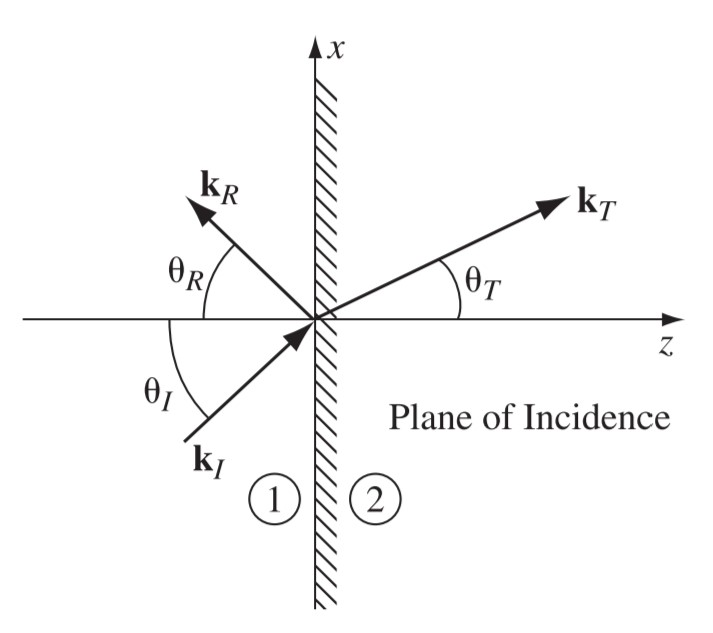
\includegraphics[width=\textwidth]{Images/re.jpg}
%             \end{figure}
%         \end{column}
%         \begin{column}{.7\linewidth}
%             \begin{beamerboxesrounded}[shadow=true]{Law of reflection}
%                 \begin{equation}
%                     \theta_I = \theta_R
%                 \end{equation}
%             \end{beamerboxesrounded}

%             \begin{beamerboxesrounded}[shadow=true]{Law of refraction (Snell's law)}
%                 \begin{equation}
%                     \frac{\sin \theta_T}{\sin \theta_I} = \frac{n_1}{n_2}
%                 \end{equation}
%             \end{beamerboxesrounded}
%             \begin{itemize}
%                 \item $n_i = v_i / c$ is called refractive index.
%                 \item When $\theta_I > \theta_{cr}$, where $\sin \theta_{cr} = n_2 / n_1$, there is a total internal reflection.
%             \end{itemize}
%         \end{column}
%     \end{columns}
% \end{frame}

% \begin{frame}{Huygens' Principle}
%     \begin{block}{Huygens' principle}
%         Every point of the wavefront may be considered as a source of secondary wavelets that propagate out in all directions with speed equal to speed of propagation of the wave.
%     \end{block}

%     \begin{figure}[htbp]
%         \centering
%         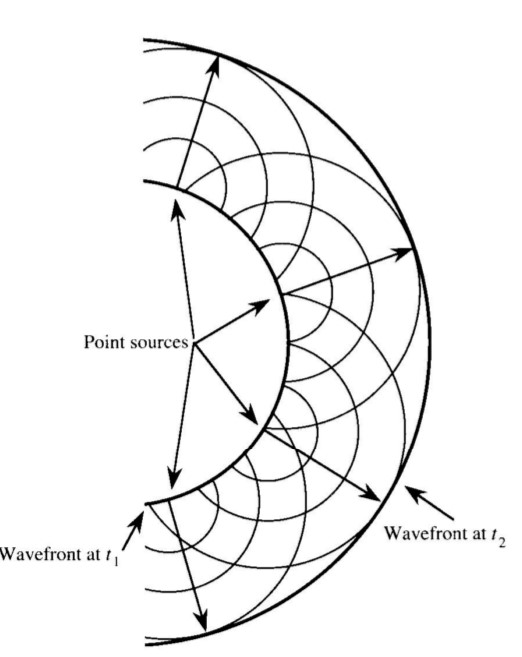
\includegraphics[height=0.5\textheight]{Images/huygens.jpg}
%     \end{figure}
% \end{frame}



\begin{frame}{Superposition of Wave Function}
    \begin{columns}
        \begin{column}{.1\linewidth}
            \begin{figure}[htbp]
                \centering
                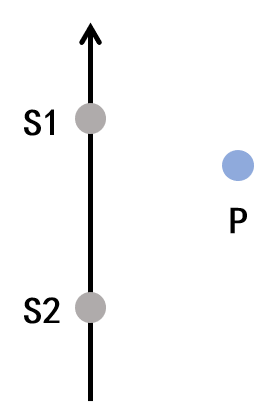
\includegraphics[width=\linewidth]{images/super.png}
                %\caption{}
                %\label{Fig:}
            \end{figure}
        \end{column}
            
        \begin{column}{.9\linewidth}
            Wave function is linear, superposition principal is applicable. 
    
    Suppose: $\mathnormal{S_1, S_2}$ in phase, same amplitude, same direction perpendicular to the plane.
    \begin{equation}
        \begin{split}
            \va{E}_1 &= \va{E}_0 \cos(kr_1-\omega t) \\
            \va{E}_2 &= \va{E}_0 \cos(kr_2-\omega t)
        \end{split}
    \end{equation}

    \begin{equation}
        \va{E}_P = \va{E}_1 + \va{E}_2 = 2\va{E}_0 \cos(\frac{k}{2}(r_1-r_2))\cos(\frac{k}{2}(r_1+r_2)-\omega t)
    \end{equation}

    \begin{itemize}
        \item Constructive interference: when $\abs{r_1-r_2}=m\lambda$
        \item Destructive interference: when $\abs{r_1-r_2}=(2m+1)\lambda/2$
    \end{itemize}
        \end{column}
    \end{columns}
    
\end{frame}

\begin{frame}{Young's Double-Slit Experiment}
    \begin{figure}[htbp]
        \centering
        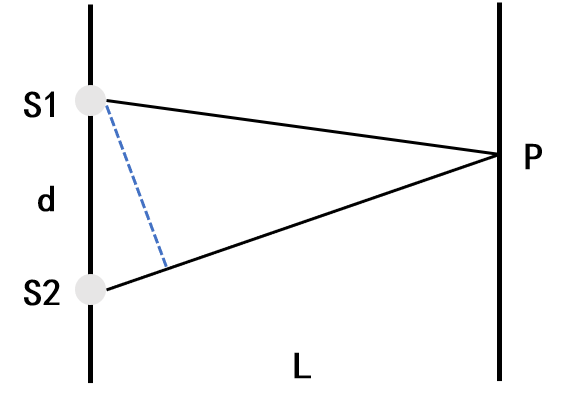
\includegraphics[scale=0.5]{images/young.png}
        %\caption{}
        %\label{Fig:}
    \end{figure}

    If $d\ll L$, $S_1-S_2\approx d\sin\theta$.
    \begin{itemize}
        \item Constructive: $\abs{r_2-r_1}=d\sin\theta_m=m\lambda$
        \item Destructive: $\abs{r_2-r_1}=d\sin\theta_m= (2m+1)\lambda/2$
        \item $\abs{y_m} = m\lambda L/d$
    \end{itemize}
\end{frame}

\begin{frame}{Interference in Thin Films}
    \begin{beamerboxesrounded}[shadow=true]{Fresnel Equations}
        \begin{equation}
            E_{reflected} = \frac{n_1\cos\theta_{incident}-n_2\cos\theta_{reflected}}{n_1\cos\theta_{incident}+n_2\cos\theta_{reflected}} E_{incident}
        \end{equation}        
        Sign changes $\Rightarrow$ phase change by $\pi (\lambda/2)$ 
    \end{beamerboxesrounded}
    \vspace{.5em}
    Other examples:
    \begin{itemize}
        \item Soap bubbles, oil specks
        \item Inclined thin films
        \item Coatings: non-reflective, reflective
        \item Newton rings (circular)
    \end{itemize}
\end{frame}

\begin{frame}{Diffraction}
    \begin{figure}[htbp]
        \centering
        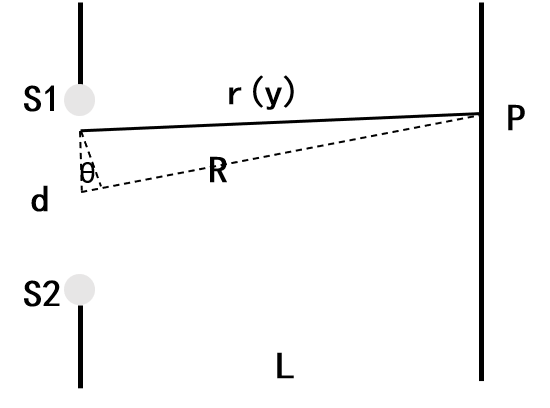
\includegraphics[scale=0.4]{images/diffraction.png}
    \end{figure} 
    
    \begin{equation}
        \begin{split}
            \tilde{E}_P &= E_0(r) \exp(i(kR-\omega t))\frac{\sin(N\delta/2)}{\sin\delta/2} \\
            \frac{I}{I_0} &= \left( \frac{\sin(N\delta/2)}{\sin\delta/2} \right)^2 
        \end{split}      
    \end{equation}

    \begin{itemize}
        \item I max: $\delta=2\pi m$, $d\sin\theta_m=\lambda m$
    \end{itemize}
\end{frame}

%----------------------------------------------------------------------------------------
%	 Section 2
%----------------------------------------------------------------------------------------

\section{Exercise}


\begin{frame}{Exercise 1}

    A source of light can generate light with continuous varying wavelengths. The light incidents a non-reflecting coating with $n_f =1.3$ vertically. It is found that the light with wavelength in vacuum: $\lambda_1= 400$ nm and $\lambda_2= 560$ nm can not be detected after the incidence, but light with all wavelengths between $\lambda_1$ and $\lambda_2$ can be detected. Please find out the thickness $t$  of the film.

    \begin{figure}[htbp]
        \centering
        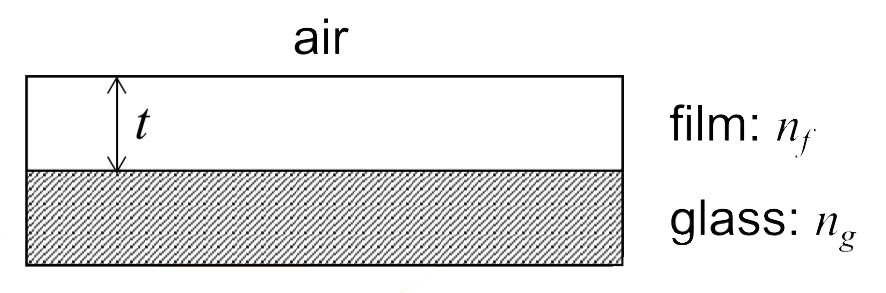
\includegraphics[width=0.7\textwidth]{Images/ex1.jpg}
    \end{figure}

\end{frame}

\begin{frame}{Exercise 2}
    A light with wavelength $\lambda=550$ nm incident vertically into Young's double slit with $d=0.2$ mm and $l=2$ m. First the system is put in air. Please find out:
    \begin{itemize}
        \item The distance between two 10-th bright fringes;
        \item If the entire system is placed in an unknown liquid, it is discovered that the position of the new 4-th bright fringe is the same as the original 3-rd bright fringe. What is the refractive index of this liquid?
    \end{itemize}

    \begin{figure}[htbp]
        \centering
        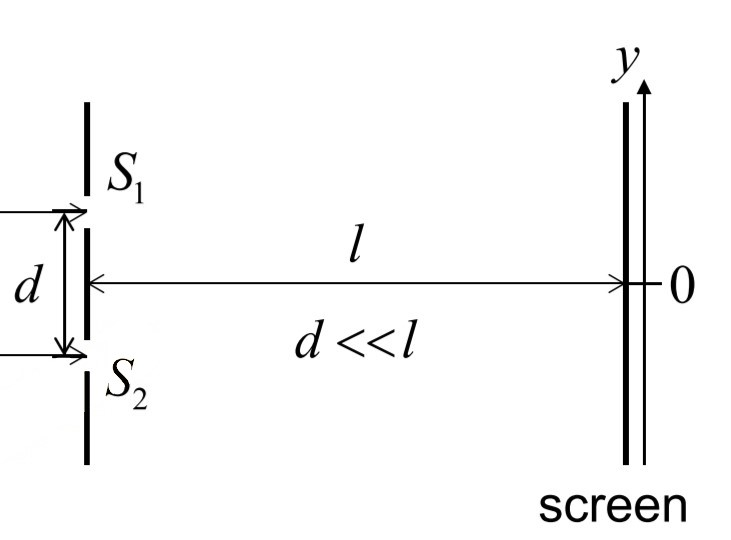
\includegraphics[width=0.45\textwidth]{Images/ex2.jpg}
    \end{figure}
\end{frame}


%	 CLOSING/SUPPLEMENTARY SLIDES
%----------------------------------------------------------------------------------------
\section{Appendix}


\begin{frame}
    \begin{center}
        \LARGE\bf Thanks for listening!
    \end{center}
\end{frame}


%----------------------------------------------------------------------------------------

\begin{frame}{\bf References}
    \nocite{*} % Display all references regardless of if they were cited
    \bibliography{example.bib}
    \bibliographystyle{plain}
\end{frame}

\end{document}

